% SIWAT user flow: six screens on the device, quick exit, and the official channels outside it.
\documentclass[border=12pt]{standalone}
\usepackage{tikz}
\usetikzlibrary{arrows.meta,positioning,calc,fit,backgrounds}
\definecolor{siwatPlum}{HTML}{38113B}
\definecolor{siwatExit}{HTML}{2B2D42}
\definecolor{siwatRed}{HTML}{E63946}
\definecolor{siwatYellow}{HTML}{E9C46A}
\definecolor{siwatGreen}{HTML}{2A9D8F}
\definecolor{siwatPaper}{HTML}{FBF7F2}
\definecolor{siwatEdge}{HTML}{DDD1DA}
\definecolor{siwatMuted}{HTML}{63506A}
\newcommand{\scr}[1]{{\ttfamily\footnotesize\bfseries\color{siwatMuted}#1}}
\renewcommand{\familydefault}{\sfdefault}
\begin{document}
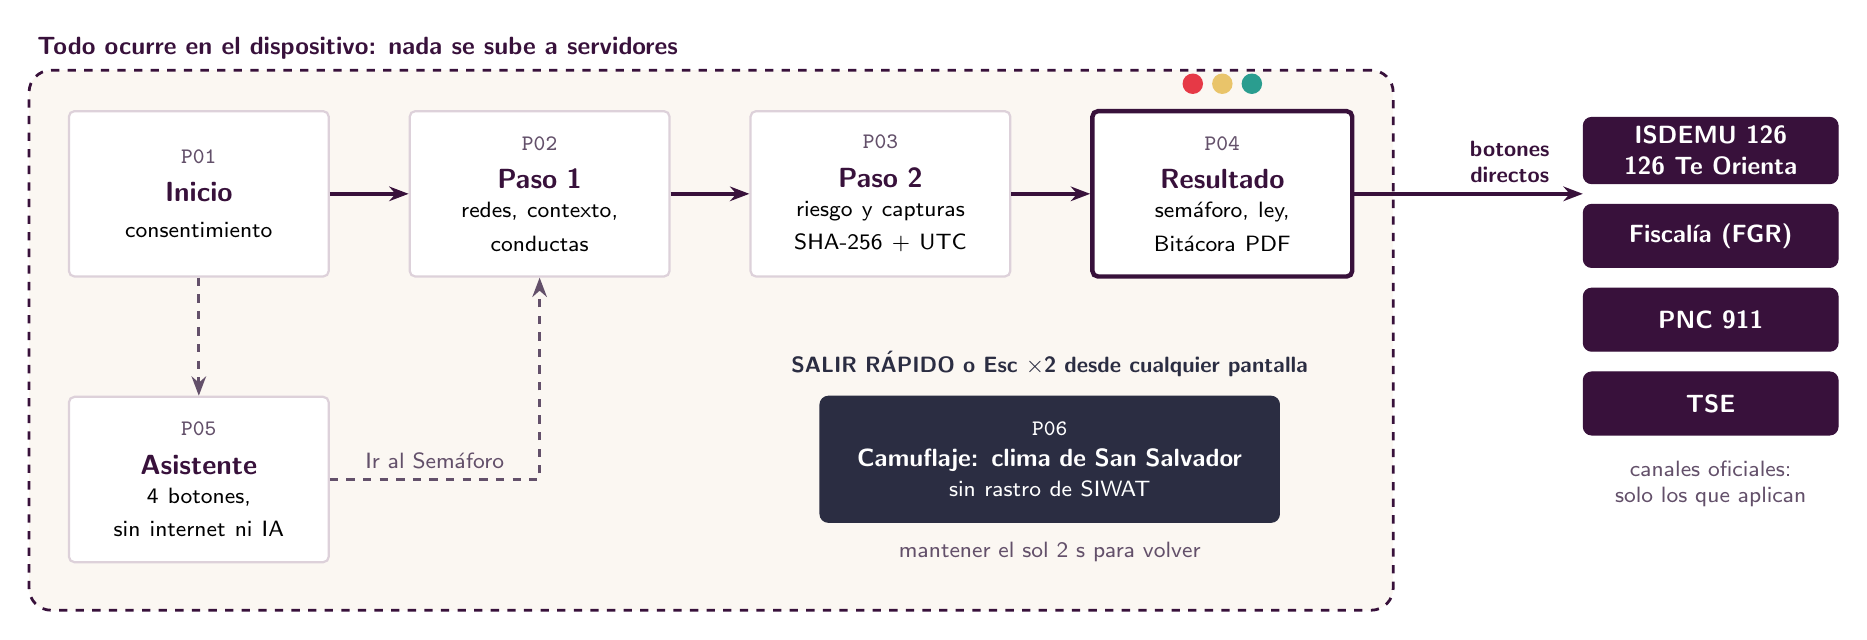
\begin{tikzpicture}[
  font=\sffamily,
  >={Stealth[length=7pt]},
  screen/.style={draw=siwatEdge, line width=0.8pt, fill=white, rounded corners=2pt,
    minimum width=3.3cm, minimum height=2.1cm, align=center, text width=3.0cm},
  flow/.style={->, line width=1.4pt, draw=siwatPlum},
  quiet/.style={->, line width=1pt, draw=siwatMuted, dashed},
  channel/.style={draw=siwatPlum, fill=siwatPlum, text=white, rounded corners=3pt,
    font=\sffamily\small\bfseries, minimum height=0.8cm, text width=3.0cm, align=center},
]
% Main path
\node[screen] (p1) {\scr{P01}\\[2pt]\textbf{\color{siwatPlum}Inicio}\\[1pt]\footnotesize consentimiento};
\node[screen, right=1.0cm of p1] (p2) {\scr{P02}\\[2pt]\textbf{\color{siwatPlum}Paso 1}\\[1pt]\footnotesize redes, contexto,\\conductas};
\node[screen, right=1.0cm of p2] (p3) {\scr{P03}\\[2pt]\textbf{\color{siwatPlum}Paso 2}\\[1pt]\footnotesize riesgo y capturas\\SHA-256 + UTC};
\node[screen, right=1.0cm of p3, draw=siwatPlum, line width=1.6pt] (p4) {\scr{P04}\\[2pt]\textbf{\color{siwatPlum}Resultado}\\[1pt]\footnotesize semáforo, ley,\\Bitácora PDF};
\draw[flow] (p1) -- (p2);
\draw[flow] (p2) -- (p3);
\draw[flow] (p3) -- (p4);

% Traffic light above the result
\foreach \c [count=\i] in {siwatRed,siwatYellow,siwatGreen}
  \fill[\c] ($(p4.north)+(-0.75+0.375*\i,0.32)$) circle (0.13);

% Assistant
\node[screen, below=1.5cm of p1] (p5) {\scr{P05}\\[2pt]\textbf{\color{siwatPlum}Asistente}\\[1pt]\footnotesize 4 botones,\\sin internet ni IA};
\draw[quiet] (p1) -- (p5);
\draw[quiet] (p5.east) -| node[pos=0.25, above, font=\footnotesize, text=siwatMuted] {Ir al Semáforo} (p2.south);

% Quick exit
\node[draw=siwatExit, fill=siwatExit, text=white, rounded corners=3pt, minimum height=1.6cm,
  text width=5.6cm, align=center, font=\sffamily\small, below=1.5cm of p3, xshift=2.15cm] (p6)
  {{\ttfamily\footnotesize\bfseries P06}\\\textbf{Camuflaje: clima de San Salvador}\\\footnotesize sin rastro de SIWAT};
\node[font=\footnotesize\bfseries, text=siwatExit, align=center, above=0.12cm of p6]
  {SALIR RÁPIDO o Esc $\times$2 desde cualquier pantalla};
\node[font=\footnotesize, text=siwatMuted, below=0.12cm of p6] (hold) {mantener el sol 2 s para volver};

% Device boundary
\begin{scope}[on background layer]
  \node[draw=siwatPlum, dashed, line width=1pt, rounded corners=8pt, fill=siwatPaper,
    inner sep=14pt, fit=(p1)(p4)(p5)(p6)(hold)] (device) {};
\end{scope}
\node[anchor=south west, font=\small\bfseries, text=siwatPlum] at (device.north west)
  {Todo ocurre en el dispositivo: nada se sube a servidores};

% Official channels, outside the device
\node[channel, right=2.9cm of p4, yshift=0.55cm] (isdemu) {ISDEMU 126\\126 Te Orienta};
\node[channel, below=0.25cm of isdemu] (fgr) {Fiscalía (FGR)};
\node[channel, below=0.25cm of fgr] (pnc) {PNC 911};
\node[channel, below=0.25cm of pnc] (tse) {TSE};
\draw[flow] (p4.east) -- node[pos=0.68, above, font=\footnotesize\bfseries, text=siwatPlum, align=center] {botones\\directos} (p4.east -| isdemu.west);
\node[font=\footnotesize, text=siwatMuted, align=center, below=0.2cm of tse] {canales oficiales:\\solo los que aplican};
\end{tikzpicture}
\end{document}
